%%%%%%%%%%%%%%%%%%%%%%%%%%%%%%%%%%%%%%%%%%%%%%%%%%%%%%%%%%%%%%%%%%%%%%%%%%%%%%%%
\chapter{Конструкторско-технологическая часть}
%%%%%%%%%%%%%%%%%%%%%%%%%%%%%%%%%%%%%%%%%%%%%%%%%%%%%%%%%%%%%%%%%%%%%%%%%%%%%%%%

%%%%%%%%%%%%%%%%%%%%%%%%%%%%%%%%%%%%%%%%%%%%%%%%%%%%%%%%%%%%%%%%%%%%%%%%%%%%%%%%
\section{Выбор технических и программных средств}
\subsection{Образовательная платформа openEDX}
OpenEDX — платформа с открытым исходным кодом. Установка осуществляется путем создания локальной копии репозитория проекта с github \cite{edx-github}. Авторы платформы предлагают запускать систему с помощью Docker \cite{docker}. Все сборки платформы будут содержать следующие компоненты \cite{edx-install}:
\begin{itemize*}
	\item программное приложения для администрирования учебных курсов (LMS);
	\item Open edX Studio;
	\item форум;
	\item систему открытого оценивания (ORA).
\end{itemize*}

Расширенные сборки также могут включать системы оплаты курсов и выдачи сертификатов, демонстрационные курсы, аналитику и другие модули. С помощью сервиса Open edX Studio можно создавать курсы. Каждый курс состоит из разделов, каждый из которых, в свою очередь, содержит один или более подразделов, сформированных блоками. 

Вид панели администратора при добавлении нового курса, наглядно демонстрирующий иерархию сущностей курса, приведен на рисунке \ref{fig:edx-structure}

\begin{figure}[htbp]
	\centering
	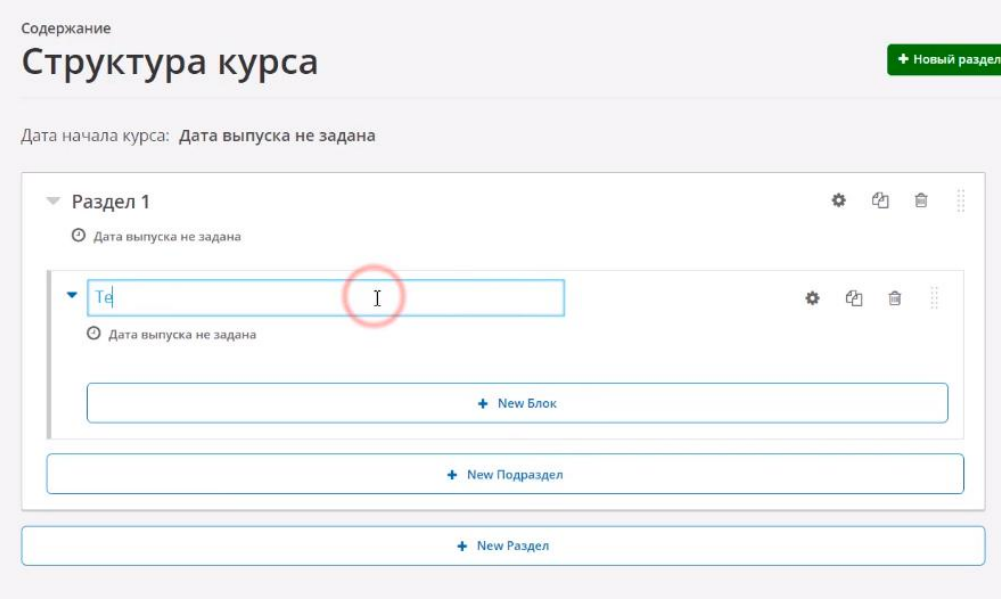
\includegraphics[width=\textwidth]{edx-structure.png}
	\caption{Иерархия сущностей курса платформы openEDX}%
	\label{fig:edx-structure}
\end{figure}

Базовая функциональность блоков разбита на четыре группы: Обсуждение, HTML, Задача и Видео. Если функции первой и последней групп очевидны, то функциональность групп Задача и HTML требуют пояснений.

Группа HTML содержит ряд инструментов для размещения содержимого в виде простого текста, опроса, объявления, текста с разворачивающимся изображением, iframe или чистого HTML. 

Группа Задача содержит набор интерактивных сценариев взаимодействия с обучающимся. Чаще всего редактирование этих сценариев осуществляется с использованием некоторого синтаксиса, напоминающего язык разметки Markdown. Пример такой задачи приведен на рисунке \ref{fig:edx-question}.


\begin{figure}[htbp]
	\centering
	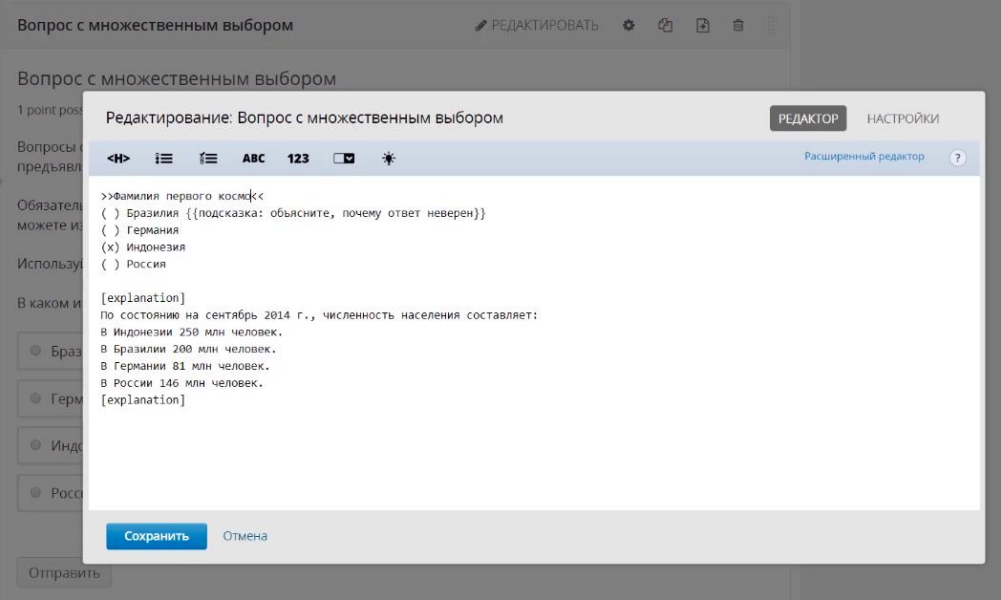
\includegraphics[width=\textwidth]{edx-question.png}
	\caption{Редактирование блока, содержащего вопрос с выбором ответа.}%
	\label{fig:edx-question}
\end{figure}

Описанная функциональность покрывает большее количество требований к образовательным курсам, однако она может быть расширена засчет добавления пользовательских компонентов, написанных с помощью технологии XBlock.

К недостаткам платформы можно отнести значительное количество кодовой базы, написанной на языке Python версии 2.7, поддержка которого в настоящее время прекращена.

\subsection{XBlock}

Для разработки пользовательских компонентов разработчики платформы предлагают собственную SDK, установка которой осуществляется также с помощью локальной копии репозитория на github \cite{sdk-github}.

Для разработки требуются python версии 2.7, виртуальное окружение venv, система
контроля версий git и СУБД SQLite.

Компоненты XBlock используют клиент-серверную архитектуру и написаны с использованием фреймворка Django. При создании нового компонента разработчику будет предложен для редактирования тестовый компонент, реализующий счетчик голосов (за и против). Файлы, подлежащие редактированию — это файл на языке python, отвечающий за серврную обработку данных, а также за подключение html-файлов шаблонов представлений, javascript-файлов, отвечающих за логику поведения на стороне клиента и css-файлов стилей.

В листинге \ref{listings:python-fields} приведен фрагмент исходного текста компонента XBlock на языке python, отвечающего за объявления полей. Для каждого поля объявляется тип данных, подсказка, значение по умолчанию и область видимости.

\lstinputlisting[
label={listings:python-fields},
caption={Объявление полей в XBlock},
style=python,
]
{listings/python-fields.txt}

Согласно документации XBlock \cite{xblock-scope}, область видимости поля - это отношение поля к пользователю и XBlock-компоненту. 

По отношению к пользователю: 

\begin{itemize*}
	\item \textbf{no user:} никакая деятельность обучающихся не влияет на данные этого поля, такие поля отображаются одинаково для всех обучающихся;
	\item \textbf{one user:} данные поля уникальны для каждого пользователя;
	\item \textbf{all users:} данные поля отображаются одинаково для всех обучающихся и могут быть модифицированы каждым из них;
\end{itemize*}

По отношению к XBlock-компоненту: 

\begin{itemize*}
	\item \textbf{block usage:} данные уникальны для каждого экземпляра XBlock;
	\item \textbf{block definition:} данные уникальны для определения, указываемого автором материала;
	\item \textbf{block type:} данные уникальны для выбранного типа XBlock, однако общие для всех его экземпляров;
	\item \textbf{all:} данные доступны всем XBlock-компонентам в системе;
\end{itemize*}

Наконец области видимости полей представляют собой комбинацию вышеперечисленных областей видимости пользователей и XBlock:
\begin{itemize*}
	\item content;
	\begin{itemize*}
		\item block definition;
		\item no user;
	\end{itemize*}
	\item settings;
	\begin{itemize*}
		\item block usage;
		\item no user;
	\end{itemize*}
	\item user\_state;
	\begin{itemize*}
		\item block usage;
		\item one user;
	\end{itemize*}
	\item preferences;
	\begin{itemize*}
		\item block type;
		\item one user;
	\end{itemize*}
	\item user\_info;
	\begin{itemize*}
		\item all blocks;
		\item one user;
	\end{itemize*}
	\item user\_state\_summary;	
	\begin{itemize*}
		\item block usage;
		\item all users;
	\end{itemize*}
\end{itemize*}

Области видимости различаются по их отношению к блокам и пользователям. Так, например, user\_info отвечает за доступ к статистике одного пользователя ко всем блокам, в
то время как user\_state\_summary — за статистику всех пользователей, использовавших
данный блок.

Для каждого из представлений, пример которого приведен в листинге \ref{listings:python-views}, создается метод, возвращающий Fragment, который содержит файл шаблона, таблицу стилей и javascript. Также указывается функция в javascript, являющаяся точкой входа в приложение, которой передается через параметры переменная окружения, корневой DOM-элемент и опции (необязательный параметр).

\lstinputlisting[
label={listings:python-views},
caption={Объявление полей в XBlock},
style=python,
]
{listings/python-views.txt}

Взаимодействие между клиентской и серверной частями приложения
осуществляется через AJAX-запросы. Обработчик объявляется с помощью аннотации
\lstinline|@XBlock.json_handler|. Пример обработчика запроса приведен в листинге \ref{listings:python-ajax}.


\lstinputlisting[
label={listings:python-ajax},
caption={Объявление полей в XBlock},
style=python,
]
{listings/python-ajax.txt}


Все отличия использования HTML-шаблонов представлений в данной структуре
заключаются в двух особенностях: во-первых, файл не имеет привычной структуры html- файла, содержащей теги \lstinline|<html>|, \lstinline||<head>| и \lstinline|<body>|, поскольку содержимое шаблона при рендеринге встраивается в уже существующую страницу. Во-вторых, в файлах шаблонов можно использовать переменные, объявленные в python-файле, обернув их в фигурные скобки. Пример файла шаблона приведен в листинге \ref{listings:html}.

\lstinputlisting[
label={listings:html},
caption={Объявление полей в XBlock},
style=html,
]
{listings/html.txt}

В листинге \ref{listings:js} приведен javascript-код XBlock-компонента. Стоит заметить, что функция обработчика запроса в python должна называться в точности так же, как URL, на
который отправляется этот запрос.

\lstinputlisting[
label={listings:js},
caption={Объявление полей в XBlock},
style=javascript,
]
{listings/js.txt}

\subsection{Javascript}

Как видно из листинга \ref{listings:js}, платформа активно использует технологию jQuery, реализующую обертки над стандартными функциями javascript, которая облегчает доступ к DOM-элементам, однако не обеспечивает двустороннего связывания данных, таким образом, не являясь гарантом консистентности модели и данных, что выливается в большие, по сравнению с современными фреймворками, трудозатраты на этапе отладки при усложнении клиентской логики.

\section{Описание системы}
\subsection{Сценарий использования}

Разрабатываемый компонент может использоваться как наглядная интерактивная иллюстрация для образовательных курсов на базе платформы openEDX, содержащих информацию как об основах программирования (переменные, ветвления, циклы), так и о базовых аспектах теории автоматического управления (ТАУ).

Ключевой сущностью компонента является робот, перемещающийся по двумерному пространству. В этом пространстве располагаются препятствия в виде отрезков (стенки) и зона успешного завершения симуляции (финиш).

Задача обучающегося — составить программу для робота таким образом, чтобы привести его к финишу, не столкнувшись со стенками. Для этого можно модифицировать такие переменные состояния робота, как его скорость и угол поворота, а также пользоваться информацией, предоставляемой его датчиками расстояния и цвета участка карты под роботом.

В свою очередь, редактор учебного материала должен настроить исходные данные таким образом, чтобы вариант решения поставленной задачи служил наглядной иллюстрацией пройденной в курсе темы.

Такими исходными данными являются:

\begin{itemize*}
	\item положение робота в пространстве (координаты x, y);
	\item начальный угол поворота робота;
	\item расположение стенок в пространстве;
	\item линии на плоскости.
\end{itemize*}

\subsection{Формальный синтаксис}
Программа для робота составляется из блоков пяти типов:
\begin{itemize*}
	\item start (старт) — точка входа в программу;
	\item instructions (инструкции) — набор команд в императивном виде, изменяющих доступные для редактирования пользователем переменные состояния робота или пользовательские переменные;
	\item condition (условие) — выражение, возвращающее логический тип данных, используемое для ветвления выполнения пользовательской программы;
	\item condition merge (слияние условия) — блок, обозначающий завершение ветвления, введенного с помощью блока condition (условие);
	\item timer (таймер) — блок, обеспечивающий задержку в выполнении пользовательской программы.
\end{itemize*}

Подробный формальный синтаксис блоков приведен в приложении.

Очевидно, блок start (старт), используемый как точка входа, должен присутствовать в программе в единичном экземпляре. По понятным причинам блок не имеет точек входа и текстового содержимого.

Блок инструкций может содержать одну или несколько команд вида \lstinline|<var> = <arithmetic expression>|, разделенных переносами строк. Здесь \lstinline|<var>| может быть как доступной для редактирования переменной состояния робота, так и пользовательской переменной. Важно отметить, что объявление пользовательских переменных, по сути, представляет собой первое упоминание такой переменной в ходе трансляции программы и может быть осуществлено только в левой части команды блока инструкций.

Поскольку все пользовательские переменные имеют глобальную область видимости на уровне javascript, однажды объявленная в рамках трансляции пользовательская переменная может быть доступна во всех последующих участках пользовательской программы. Так, по причине того, что цепочка блоков, расположенная между блоками condition (условие) и condition merge (слияние условия), подлежащая исполнению в случае, когда результатом вычисления выражения блока условия является логическая истина, транслируется раньше, чем цепочка, подлежащая выполнению в противоположном случае, пользовательская переменная, объявленная в первой цепочке, может использоваться в правых частях выражений блока инструкций и блоках условий второй цепочки, однако данная практика является примером плохого стиля написания кода и не рекомендуется к использованию.  

\subsection{Трансляция программы}

Результатом трансляции программы являются два массива: массив экранированных пользовательских переменных и массив инструкций для модуля исполнения программы.

Инструкции представляют собой объекты javascript с обязательными ключами «тип» и «текст». В случае инструкции «condition» добавляется информация о блоке и адресе первой инструкции «ложной ветки», для «instruction» — информация о блоке и строке. Дополнительные поля нужны для обеспечения подробной информации об ошибках времени выполнения.

По сути, допустимый код пользовательской программы представляет собой подмножество языка javascript, который проверяется транслятором на соответствие формальному синтаксису разработанного языка и подставляется в поле «текст» результирующей инструкции с подстановкой реальных переменных состояния робота вместо их псевдонимов и экранированием пользовательских переменных с целью избежания их пересечения с глобальными переменными, используемыми на странице курса.

Каждая непустая строка блока инструкций преобразуется в команду «instruction», блок условия — в команду «condition», таймера — в «timer». Ветвление пользовательской программы осуществляется с помощью инструкции «jump».

Блок-схема алгоритма работы транслятора приведена на рисунке \ref{fig:translator-scheme}.

\begin{figure}[htbp]
	\centering
	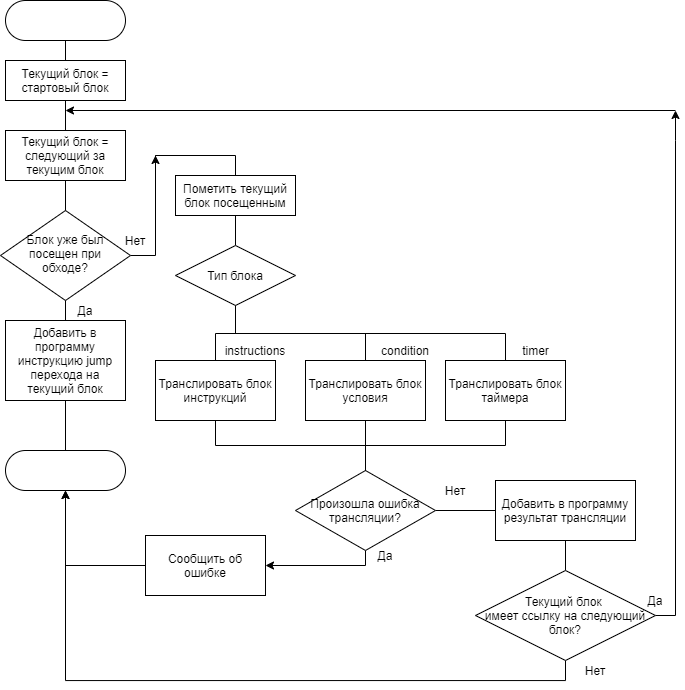
\includegraphics[width=\textwidth]{translator-scheme.png}
	\caption{Схема алгоритма работы транслятора}%
	\label{fig:translator-scheme}
\end{figure}

\subsection{Выполнение программы}

В начале этапа выполнения программы происходит инициализация пользовательских переменных. Для каждой переменной \lstinline|v| выполняется \lstinline|window[v] = 0|. Переменная явно инициализируется типом Number для экономии ресурсов, поскольку формальный синтаксис использует оператор «==» в качестве оператора равенства, который для сравнения приводит типы операндов к общему, в случае, если они не совпадают \cite{mdn-sameness}.

Затем, инициализируется счетчик команд \lstinline|this.PC = 0| и запускается цикл выполнения. В этом цикле каждая инструкция помещается в очередь задач с помощью  функции \lstinline|setInterval| с параметром задержки, равном нулю. Такая реализация позволяет параллельно работать модулям выполнения программы и отрисовки модели, не блокируя при этом выполнение сценариев на остальной странице.

Реализация таймера представляет собой отмену цикла выполнения через \lstinline|clearInterval|, с последующим его возобновлением с помощью \lstinline|setTimeout| с параметром задержки, равному содержимому блока «timer».

Цикл выполнения считается завершенным при выходе счетчика команд за границы массива, что, однако не означает окончание процесса симуляции. Так, например, если выполнение программы завершилось, но переменная состояние робота имеет значение, отличное от нуля, робот продолжит движение в заданном направлении, пока не придет либо в область финиша (успешное окончание симуляции), либо не пересечется со стенкой (неуспешное окончание симуляции).

 
\section{Пользовательский интерфейс}

%%%%%%%%%%%%%%%%%%%%%%%%%%%%%%%%%%%%%%%%%%%%%%%%%%%%%%%%%%%%%%%%%%%%%%%%%%%%%%%%
